% Architecture diagram: pdflatex architecture.tex  (writes architecture.pdf; architecture.png via pdftoppm)
\documentclass[border=6pt]{standalone}
\usepackage[T1]{fontenc}
\usepackage{helvet}
\renewcommand{\familydefault}{\sfdefault}
\usepackage{tikz}
\usetikzlibrary{arrows.meta,positioning,fit,backgrounds,calc}

\definecolor{ink}{HTML}{0F2A1D}
\definecolor{green}{HTML}{15803D}
\definecolor{greensoft}{HTML}{ECFDF3}
\definecolor{blue}{HTML}{1D4ED8}
\definecolor{bluesoft}{HTML}{EFF4FF}
\definecolor{amber}{HTML}{B45309}
\definecolor{ambersoft}{HTML}{FFF7E6}
\definecolor{grey}{HTML}{64748B}
\definecolor{band}{HTML}{F6F7F5}

\begin{document}
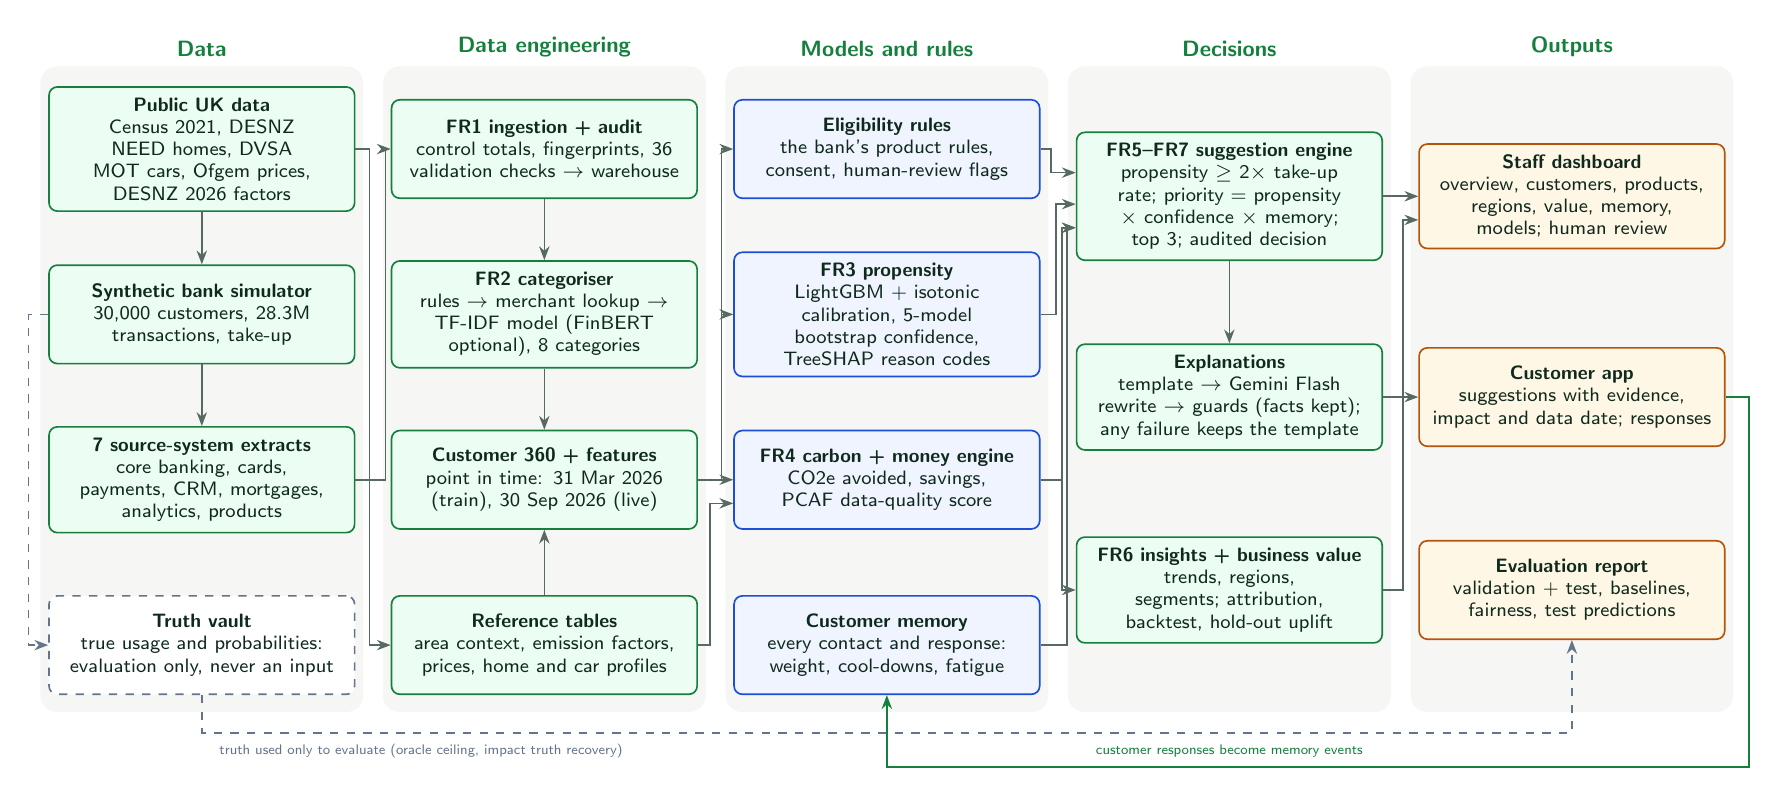
\begin{tikzpicture}[
  font=\scriptsize, text=ink, >={Stealth[length=5pt]},
  box/.style={draw=green, fill=greensoft, rounded corners=3pt, line width=0.6pt, text width=3.6cm, align=center,
              execute at begin node={\hyphenpenalty=10000\exhyphenpenalty=10000},
              inner sep=4pt, minimum height=1.25cm},
  model/.style={box, draw=blue, fill=bluesoft},
  outbox/.style={box, draw=amber, fill=ambersoft},
  hidden/.style={box, draw=grey, fill=white, dashed},
  flow/.style={->, line width=0.6pt, draw=ink!70},
  evalflow/.style={->, line width=0.6pt, draw=grey, dashed},
  head/.style={font=\footnotesize\bfseries, text=green, anchor=south},
]
\def\dx{4.35}

% ---- column 1: data
\node[box]    (pub)   at (0,0)      {\textbf{Public UK data}\\Census 2021, DESNZ NEED homes, DVSA MOT cars, Ofgem prices, DESNZ 2026 factors};
\node[box]    (sim)   at (0,-2.1)   {\textbf{Synthetic bank simulator}\\30,000 customers, 28.3M transactions, take-up};
\node[box]    (src)   at (0,-4.2)   {\textbf{7 source-system extracts}\\core banking, cards, payments, CRM, mortgages, analytics, products};
\node[hidden] (truth) at (0,-6.3)   {\textbf{Truth vault}\\true usage and probabilities: evaluation only, never an input};

% ---- column 2: data engineering
\node[box]    (fr1)   at (\dx,0)    {\textbf{FR1 ingestion + audit}\\control totals, fingerprints, 36 validation checks $\rightarrow$ warehouse};
\node[box]    (fr2)   at (\dx,-2.1) {\textbf{FR2 categoriser}\\rules $\rightarrow$ merchant lookup $\rightarrow$ TF-IDF model (FinBERT optional), 8 categories};
\node[box]    (c360)  at (\dx,-4.2) {\textbf{Customer 360 + features}\\point in time: 31 Mar 2026 (train), 30 Sep 2026 (live)};
\node[box]    (ref)   at (\dx,-6.3) {\textbf{Reference tables}\\area context, emission factors, prices, home and car profiles};

% ---- column 3: models and rules
\node[model]  (elig)  at (2*\dx,0)    {\textbf{Eligibility rules}\\the bank's product rules, consent, human-review flags};
\node[model]  (fr3)   at (2*\dx,-2.1) {\textbf{FR3 propensity}\\LightGBM + isotonic calibration, 5-model bootstrap confidence, TreeSHAP reason codes};
\node[model]  (fr4)   at (2*\dx,-4.2) {\textbf{FR4 carbon + money engine}\\CO2e avoided, savings, PCAF data-quality score};
\node[model]  (mem)   at (2*\dx,-6.3) {\textbf{Customer memory}\\every contact and response: weight, cool-downs, fatigue};

% ---- column 4: decisions
\node[box]    (rec)   at (3*\dx,-0.6) {\textbf{FR5--FR7 suggestion engine}\\propensity $\geq$ 2$\times$ take-up rate; priority = propensity $\times$ confidence $\times$ memory; top 3; audited decision};
\node[box]    (exp)   at (3*\dx,-3.15) {\textbf{Explanations}\\template $\rightarrow$ Gemini Flash rewrite $\rightarrow$ guards (facts kept); any failure keeps the template};
\node[box]    (val)   at (3*\dx,-5.6) {\textbf{FR6 insights + business value}\\trends, regions, segments; attribution, backtest, hold-out uplift};

% ---- column 5: outputs
\node[outbox]    (staff) at (4*\dx,-0.6) {\textbf{Staff dashboard}\\overview, customers, products, regions, value, memory, models; human review};
\node[outbox]    (app)   at (4*\dx,-3.15) {\textbf{Customer app}\\suggestions with evidence, impact and data date; responses};
\node[outbox]    (evr)   at (4*\dx,-5.6) {\textbf{Evaluation report}\\validation + test, baselines, fairness, test predictions};

% ---- column bands and headers
\begin{scope}[on background layer]
  \foreach \c/\n in {0/c1,1/c2,2/c3,3/c4,4/c5} {
    \fill[band, rounded corners=6pt] ($(\c*\dx,0)+(-2.05,1.05)$) rectangle ($(\c*\dx,-6.3)+(2.05,-0.85)$);
  }
\end{scope}
\node[head] at (0,1.05)      {Data};
\node[head] at (\dx,1.05)    {Data engineering};
\node[head] at (2*\dx,1.05)  {Models and rules};
\node[head] at (3*\dx,1.05)  {Decisions};
\node[head] at (4*\dx,1.05)  {Outputs};

% ---- flows
\draw[flow] (pub) -- (sim);
\draw[flow] (sim) -- (src);
\draw[evalflow] (sim.west) -- ++(-0.25,0) |- (truth.west);
\draw[flow] (src.east) -- ++(0.38,0) |- (fr1.west);
\draw[flow] (fr1) -- (fr2);
\draw[flow] (fr2) -- (c360);
\draw[flow] (pub.east) -- ++(0.18,0) |- (ref.west);
\draw[flow] (ref) -- (c360);
\draw[flow] (c360.east) -- ++(0.3,0) |- (elig.west);
\draw[flow] (c360.east) -- ++(0.3,0) |- (fr3.west);
\draw[flow] (c360) -- (fr4);
\draw[flow] (ref.east) -- ++(0.15,0) |- ($(fr4.west)+(0,-0.3)$);
\draw[flow] (elig.east) -- ++(0.13,0) |- ($(rec.west)+(0,0.3)$);
\draw[flow] (fr3.east) -- ++(0.2,0) |- ($(rec.west)+(0,-0.1)$);
\draw[flow] (fr4.east) -- ++(0.27,0) |- ($(rec.west)+(0,-0.4)$);
\draw[flow] (mem.east) -- ++(0.34,0) |- ($(rec.west)+(0,-0.4)$);
\draw[flow] (rec) -- (exp);
\draw[flow] (rec) -- (staff);
\draw[flow] (exp) -- (app);
\draw[flow] (fr4.east) -- ++(0.27,0) |- (val.west);
\draw[flow] (val.east) -- ++(0.25,0) |- ($(staff.west)+(0,-0.3)$);
\draw[flow, draw=green] (app.east) -- ++(0.3,0) |- (2*\dx,-7.85) -- (mem.south);
\node[font=\tiny, text=green, anchor=south] at (3*\dx,-7.85) {customer responses become memory events};
\draw[evalflow] (truth.south) -- ++(0,-0.48) -| (evr.south);
\node[font=\tiny, text=grey, anchor=north west] at ($(truth.south)+(0.1,-0.5)$) {truth used only to evaluate (oracle ceiling, impact truth recovery)};
\end{tikzpicture}
\end{document}
